\chapter{Lattice Element Types}
\label{c:ele.types}

%---------------------------------------------------------------------------------------------------

This chapter discusses the various types of elements
available in \accellat.
These elements are:
\begin{table}[htb]
\centering
{\tt
\begin{tabular}{llll} \toprule
  {\it Element}     & {\it Section}         & {\it Element}      & {\it Section}      \\ \midrule
  ACKicker          & \ref{s:ackicker}      &  Marker           & \ref{s:marker}      \\
  BeamBeam          & \ref{s:beambeam}      &  Mask             & \ref{s:mask}        \\
  BeginningEle      & \ref{s:begin.ele}     &  Match            & \ref{s:match}       \\
  Bend              & \ref{s:bend}          &  Multipole        & \ref{s:mult}        \\
  Converter         & \ref{s:converter}     &  NullEle          & \ref{s:nullele}     \\
  Collimator        & \ref{s:collimator}    &  Octupole         & \ref{s:octupole}    \\
  CrabCavity        & \ref{s:crabcavity}    &  Patch            & \ref{s:patch}       \\
  Drift             & \ref{s:drift}         &  Quadrupole       & \ref{s:quadrupole}  \\
  EGun              & \ref{s:egun}          &  RFCavity         & \ref{s:rfcavity}    \\
  Fiducial          & \ref{s:fiducial}      &  Sextupole        & \ref{s:sextupole}   \\
  FloorShift        & \ref{s:floorshift}    &  Solenoid         & \ref{s:solenoid}    \\
  Foil              & \ref{s:foil}          &  Taylor           & \ref{s:taylor}      \\
  Fork              & \ref{s:fork}          &  ThickMultipole   & \ref{s:thickmult}   \\
  Girder            & \ref{s:girder}        &  Undulator        & \ref{s:undulator}   \\
  Instrument        & \ref{s:instrument}    &  UnionEle         & \ref{s:unionele}    \\
  Kicker            & \ref{s:kicker}        &  Wiggler          & \ref{s:wiggler}     \\
  LCavity           & \ref{s:lcavity}       &                   &                     \\
  \bottomrule
\end{tabular}
} 
\caption{Table of element types.}
\label{t:particle.classes}
\end{table}

\newpage

%---------------------------------------------------------------------------------------------------
\section{ACKicker}
\label{s:ackicker}

An \vn{ac_kicker} element simulates a ``slow'' time dependent kicker element.

NOTE: This Element is in development and is incomplete. 
Missing: Need to document amp_function function to return the kick amplitude.

Element parameter groups associated with this element type are:
\TOPrule 
\begin{example}
  BodyShiftParams     -> Element position/orientation shift. \sref{s:align.g} 
  ApertureParams      -> Vacuum chamber aperture. \sref{s:aperture.g} 
  BMultipoleParams    -> Magnetic multipoles. \sref{s:bmultipole.g} 
  FloorParams -> Floor floor position and orientation. \sref{s:orientation.g} 
  LengthParams        -> Length and s-position parameters. \sref{s:length.g} 
  LordSlaveParams     -> Element lord and slave status. \sref{s:lord.slave.g} 
  MasterParams        -> Contains field_master parameter. \sref{s:master.g} 
  DescriptionParams   -> Element descriptive strings. \sref{s:descrip.g} 
  TrackingParams      -> Default tracking settings. \sref{s:tracking.g} 
  ReferenceParams     -> Reference energy and species. \sref{s:reference.g}
  DownstreamReferenceParams -> Reference energy and species at downstream end. \sref{s:dreference.g}
\end{example}
\BOTTOMrule


The calculated field will only obey Maxwell's equations in the limit that the time variation
of the field is ``slow'':
\begin{equation}
  \omega \ll \frac{c}{r}
\end{equation}
where $\omega$ is the characteristic frequency of the field variation, $c$ is the speed of light,
and $r$ is the characteristic size of the \vn{ACKicker} element. That is, the fields at opposite
ends of the element must be able to ``communicate'' (which happens at the speed of light) in a time
scale short compared to the time scale of the change in the field.

\newpage

%---------------------------------------------------------------------------------------------------
\section{BeamBeam}
\label{s:beambeam}

A \vn{beambeam} element simulates an interaction with an opposing
(``strong'') beam traveling in the opposite direction.

NOTE: This Element is in development and is incomplete

Element parameter groups associated with this element type are:
\TOPrule
\begin{example}
  FloorParams -> Floor floor position and orientation. \sref{s:orientation.g} 
  LengthParams        -> Length and s-position parameters. \sref{s:length.g} 
  LordSlaveParams     -> Element lord and slave status. \sref{s:lord.slave.g} 
  DescriptionParams   -> Element descriptive strings. \sref{s:descrip.g} 
  TrackingParams      -> Default tracking settings. \sref{s:tracking.g} 
  ReferenceParams     -> Reference energy and species. \sref{s:reference.g}
  DownstreamReferenceParams -> Reference energy and species at downstream end. \sref{s:dreference.g}
\end{example}
\BOTTOMrule


\newpage

%---------------------------------------------------------------------------------------------------
\section{BeginningEle}
\label{s:begin.ele}

A \vn{BeginningEle} element must be present as the first element of every tracking branch.
(\sref{s:branch.def}).

Element parameter groups associated with this element type are:
\TOPrule
\begin{example}
  FloorParams -> Floor floor position and orientation. \sref{s:orientation.g} 
  InitParticleParams  -> Initial particle position and spin. \sref{s:init.particle.g} 
  LengthParams        -> Length and s-position parameters. \sref{s:length.g} 
  LordSlaveParams     -> Element lord and slave status. \sref{s:lord.slave.g} 
  DescriptionParams   -> Element descriptive strings. \sref{s:descrip.g} 
  TrackingParams      -> Default tracking settings. \sref{s:tracking.g} 
  TwissParams         -> Initial Twiss and coupling parameters. \sref{s:twiss.g} 
  ReferenceParams     -> Reference energy and species. \sref{s:reference.g}
  DownstreamReferenceParams -> Reference energy and species at downstream end. \sref{s:dreference.g}
\end{example}
\BOTTOMrule


Example:
\begin{example}
  @ele bg = BeginningEle(species_ref = Species("proton"), pc_ref = 1e11)
\end{example}

\newpage

%---------------------------------------------------------------------------------------------------
\section{Bend}
\label{s:bend}

A \vn{Bend} element represents a dipole bend. Bends have a design bend angle and bend radius
which determines the location of downstream elements as documented in \sref{s:branch.coords}.
The actual bending strength that a particle feels can differ from the design value as detailed
below.

Element parameter groups associated with this element type are:
\TOPrule
\begin{example}
  BodyShiftParams     -> Element position/orientation shift. \sref{s:align.g} 
  ApertureParams      -> Vacuum chamber aperture. \sref{s:aperture.g} 
  BMultipoleParams    -> Magnetic multipoles. \sref{s:bmultipole.g} 
  BendParams          -> Bend element parameters. \sref{s:bend.g} 
  EMultipoleParams    -> Electric multipoles. \sref{s:emultipole.g} 
  FloorParams -> Floor floor position and orientation. \sref{s:orientation.g} 
  LengthParams        -> Length and s-position parameters. \sref{s:length.g} 
  LordSlaveParams     -> Element lord and slave status. \sref{s:lord.slave.g} 
  MasterParams        -> Contains field_master parameter. \sref{s:master.g} 
  DescriptionParams   -> Element descriptive strings. \sref{s:descrip.g} 
  TrackingParams      -> Default tracking settings. \sref{s:tracking.g} 
  ReferenceParams     -> Reference energy and species. \sref{s:reference.g}
  DownstreamReferenceParams -> Reference energy and species at downstream end. \sref{s:dreference.g}
\end{example}
\BOTTOMrule


\begin{figure}[ht]
  \centering 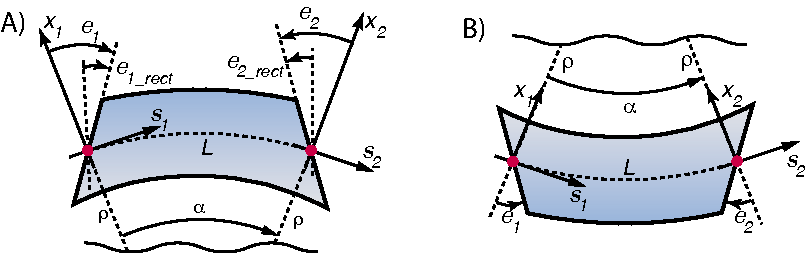
\includegraphics{bend.pdf} 
\caption[Bend geometry]{
Bend geometry. Red dots are the entry and exit points that define the origin for the
coordinate systems at the entry end $(s_1, x_1)$ and exit ends $(s_2, x_2)$ respectively. 
In the figure, the angle \vn{alpha} is denoted $\alpha$ and the radius
\vn{rho} is denoted $\rho$.
A) Bend geometry with positive bend angle. For the geometry shown, 
\vn{g}, \vn{angle}, \vn{rho}, \vn{e1}, \vn{e2}, \vn{e1_rect}, and \vn{e2_rect} are all positive.
B) Bend geometry with negative bend angle. For the geometry shown, 
\vn{g}, \vn{angle}, \vn{rho}, \vn{e1}, \vn{e2}, \vn{e1_rect}, and \vn{e2_rect} are all negative.
Note: The figures are drawn for zero \vn{ref_tilt} where the rotation axis is parallel to the 
$y$-axis. 
}
\label{f:bend2}
\end{figure}

The \vn{BendParams} group (\sref{s:bend.g}) contains the parameters that define the shape of the bend.

Example:
\begin{example}
  @ele b03w = Bend(l = 0.6, g = 0.017, kn1 = 0.003)
\end{example}

\newpage

%---------------------------------------------------------------------------------------------------
\section{Collimator}
\label{s:collimator}

\vn{Collimators} are field free elements that can collimate beam particles.

Element parameter groups associated with this element type are:
\TOPrule
\begin{example}
  FloorParams -> Floor floor position and orientation. \sref{s:orientation.g} 
  LengthParams        -> Length and s-position parameters. \sref{s:length.g} 
  LordSlaveParams     -> Element lord and slave status. \sref{s:lord.slave.g} 
  DescriptionParams   -> Element descriptive strings. \sref{s:descrip.g} 
  TrackingParams      -> Default tracking settings. \sref{s:tracking.g} 
  ReferenceParams     -> Reference energy and species. \sref{s:reference.g}
  DownstreamReferenceParams -> Reference energy and species at downstream end. \sref{s:dreference.g}
\end{example}
\BOTTOMrule

%---------------------------------------------------------------------------------------------------
\section{Converter}
\label{s:converter}

\vn{Converter} elements convert from one particle species to another. 
For example, converting electrons hitting on a metal target into positrons.

NOTE: This Element is in development and is incomplete.

Element parameter groups associated with this element type are:
\TOPrule
\begin{example}
  FloorParams -> Floor floor position and orientation. \sref{s:orientation.g} 
  LengthParams        -> Length and s-position parameters. \sref{s:length.g} 
  LordSlaveParams     -> Element lord and slave status. \sref{s:lord.slave.g} 
  DescriptionParams   -> Element descriptive strings. \sref{s:descrip.g} 
  TrackingParams      -> Default tracking settings. \sref{s:tracking.g} 
  ReferenceParams     -> Reference energy and species. \sref{s:reference.g}
  DownstreamReferenceParams -> Reference energy and species at downstream end. \sref{s:dreference.g}
\end{example}
\BOTTOMrule

%---------------------------------------------------------------------------------------------------
\section{CrabCavity}
\label{s:crabcavity}

A \vn{CrabCavity} is an RF cavity that gives a $z$-dependent transverse kick. 
This is useful in colliding beam machines, where there is a finite crossing angle at the 
interaction point, to rotate the beams near the IP.

NOTE: This Element is in development and is incomplete.

Element parameter groups associated with this element type are:
\TOPrule
\begin{example}
  FloorParams -> Floor floor position and orientation. \sref{s:orientation.g} 
  LengthParams        -> Length and s-position parameters. \sref{s:length.g} 
  LordSlaveParams     -> Element lord and slave status. \sref{s:lord.slave.g} 
  DescriptionParams   -> Element descriptive strings. \sref{s:descrip.g} 
  TrackingParams      -> Default tracking settings. \sref{s:tracking.g} 
  ReferenceParams     -> Reference energy and species. \sref{s:reference.g}
  DownstreamReferenceParams -> Reference energy and species at downstream end. \sref{s:dreference.g}
\end{example}
\BOTTOMrule


%---------------------------------------------------------------------------------------------------
\section{Drift}
\label{s:drift}

A \vn{Drift} is a field free element.

Element parameter groups associated with this element type are:
\TOPrule
\begin{example}
  FloorParams -> Floor floor position and orientation. \sref{s:orientation.g} 
  LengthParams        -> Length and s-position parameters. \sref{s:length.g} 
  LordSlaveParams     -> Element lord and slave status. \sref{s:lord.slave.g} 
  DescriptionParams   -> Element descriptive strings. \sref{s:descrip.g} 
  TrackingParams      -> Default tracking settings. \sref{s:tracking.g} 
  ReferenceParams     -> Reference energy and species. \sref{s:reference.g}
  DownstreamReferenceParams -> Reference energy and species at downstream end. \sref{s:dreference.g}
\end{example}
\BOTTOMrule

%---------------------------------------------------------------------------------------------------
\section{EGun}
\label{s:egun}

An \vn{EGun} element represents an electron gun and encompasses a region starting from the cathode
were the electrons are generated.  

NOTE: This Element is in development and is incomplete.

Element parameter groups associated with this element type are:
\TOPrule
\begin{example}
  FloorParams -> Floor floor position and orientation. \sref{s:orientation.g} 
  LengthParams        -> Length and s-position parameters. \sref{s:length.g} 
  LordSlaveParams     -> Element lord and slave status. \sref{s:lord.slave.g} 
  DescriptionParams   -> Element descriptive strings. \sref{s:descrip.g} 
  TrackingParams      -> Default tracking settings. \sref{s:tracking.g} 
  ReferenceParams     -> Reference energy and species. \sref{s:reference.g}
  DownstreamReferenceParams -> Reference energy and species at downstream end. \sref{s:dreference.g}
\end{example}
\BOTTOMrule

%---------------------------------------------------------------------------------------------------
\section{Fiducial}
\label{s:fiducial}

A \vn{Fiducial} element is used to fix the position and orientation of the reference orbit within
the floor coordinate system at the location of the \vn{Fiducial} element. A \vn{Fiducial} element
will affect the floor floor coordinates (\sref{s:floor}) of elements both upstream and downstream
of the fiducial element.

NOTE: This Element is in development and is incomplete.

Element parameter groups associated with this element type are:
\TOPrule
\begin{example}
  FloorParams -> Floor floor position and orientation. \sref{s:orientation.g} 
  LengthParams        -> Length and s-position parameters. \sref{s:length.g} 
  LordSlaveParams     -> Element lord and slave status. \sref{s:lord.slave.g} 
  DescriptionParams   -> Element descriptive strings. \sref{s:descrip.g} 
  TrackingParams      -> Default tracking settings. \sref{s:tracking.g} 
  ReferenceParams     -> Reference energy and species. \sref{s:reference.g}
  DownstreamReferenceParams -> Reference energy and species at downstream end. \sref{s:dreference.g}
\end{example}
\BOTTOMrule


%---------------------------------------------------------------------------------------------------
\section{FloorShift}
\label{s:floorshift}

A \vn{FloorShift} element shifts the reference orbit in the floor coordinate system without
affecting particle tracking. That is, in terms of tracking, a \vn{FloorShift} element is equivalent
to a \vn{Marker} (\sref{s:marker}) element. 

NOTE: This Element is in development and is incomplete.

%---------------------------------------------------------------------------------------------------
\section{Foil}
\label{s:foil}

A \vn{Foil} element represents a planar sheet of material which can strip electrons from a particle.
In conjunction, there will be scattering of the particle trajectory as well as an associated energy
loss.

NOTE: This Element is in development and is incomplete.

%---------------------------------------------------------------------------------------------------
\section{Fork}
\label{s:fork}

\begin{figure}[tb]
  \centering
  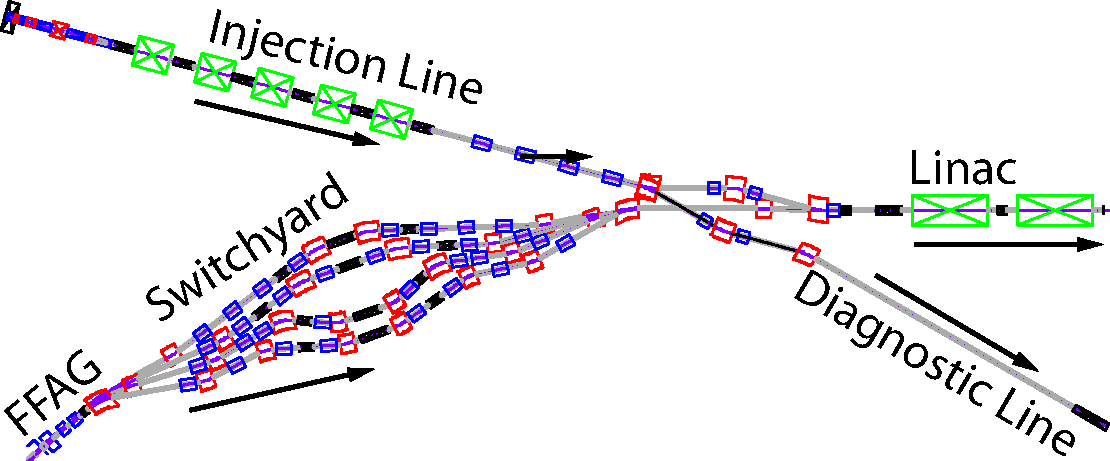
\includegraphics[width=5in]{fork-patch.pdf}
  \caption[Cornell/Brookhaven CBETA ERL/FFAG machine with fork elements.]
  {
Section of the 8-pass (4 passes with increasing energy and 4 passes with decreasing energy) 
Cornell/Brookhaven CBETA ERL/FFAG machine. Fork elements are used to connect the 
injection line to the ring and to connect the ring to a diagnostic line. The geometry of the
switchyard, used to correct the timings of the differing energy beams, is done using Patch elements.
  }
  \label{f:fork.cbeta}
\end{figure}

A \vn{Fork} element marks a branching point in a lattice branch. Examples include \vn{Fork} from
a ring to an extraction line or an X-ray beam line, or \vn{Fork} from the end of an injection line to
someplace in a ring. An example is shown in \fig{f:fork.cbeta}.

Element parameter groups associated with this element type are:
\TOPrule
\begin{example}
  FloorParams -> Floor floor position and orientation. \sref{s:orientation.g} 
  LengthParams        -> Length and s-position parameters. \sref{s:length.g} 
  DescriptionParams   -> Element descriptive strings. \sref{s:descrip.g} 
  TrackingParams      -> Default tracking settings. \sref{s:tracking.g} 
  ForkParams          -> Fork parameters. \sref{s:fork.g}
  ReferenceParams     -> Reference energy and species. \sref{s:reference.g}
  DownstreamReferenceParams -> Reference energy and species at downstream end. \sref{s:dreference.g}
\end{example}
\BOTTOMrule

The \vn{branch} containing a \vn{Fork} element is called the
``\vn{base} \vn{branch}''. The \vn{branch} that the \vn{Fork} element points to is called the
``\vn{forked-to} \vn{branch}''. The to_ele...

Fork elements may be put in a lattice by including them in beamlines before a lattice
is instantiated. After a lattice has been instantiated, Fork elements can be inserted
by using the \vn{superimpose!} or \vn{insert!} functions.

The components of this group are:
\begin{example}
  to_line::Union{BeamLine,Branch}   - Beam line to fork to
  to_ele::Union{String,Ele}         - Element forked to.
  direction::Int                    - Longitudinal Direction of injected beam.
\end{example}






If a fork creates a new branch, and if the The reference energy or species type for the forked-to branch is the particle 
particle associated with a branch can be set by setting the \vn{particle} attribute of the \vn{Fork}
element.


\index{patch}
Forked-to branches can themselves have \vn{Fork} elements. A branch always starts out tangential to the
line it is branching from.  A \vn{patch} element (\sref{s:patch}) can be used to reorient the
reference orbit as needed. Example:
\begin{example}
  @ele x_patch = Patch,(offset[1] = 0.01)
  @ele pb = Fork(to_line = x_line)
  @ele bgn = BeginningEle(p0c = 1e3, species_ref = Species("photon")
                                                  ! Photon reference momentum   
  from_line = BeamLine([... a, pb, b, ...])       ! Defines base branch
  x_line = BeamLine([bgn, x_patch, x1, x2, ...])  ! Defines forked-to branch
\end{example}
In this example, a photon generated at the fork element \vn{pb} with $x = 0$ with respect to the
\vn{from_line} reference orbit through \vn{pb} will, when transferred to the \vn{x_line}, and
propagated through \vn{x_patch}, have an initial value for $x$ of $-0.01$.

Forking elements have zero length and, like \vn{Marker} elements, the position of a particle tracked
through a \vn{Fork} element does not change.

Forking elements do not have orientational attributes like \vn{x_pitch} and \vn{tilt}
(\ref{s:offset}). If the orientation of the forked-to branch needs to be modified, this can be
accomplished using a \vn{patch} element at the beginning of the line.

\index{is_on}
The \vn{is_on} attribute, while provided for use by a program, is ignored by \bmad proper.

If the reference orbit needs to be shifted when \vn{Fork} from one ring to another ring, a patch can
be placed in a separate ``transfer'' line to isolate it from the branches defining the
rings. Example:
\begin{example}
  ring1: line = (... A, F1, B, ...)     ! First ring
  x_line: line = (X_F1, X_PATCH, X_F2)  ! "Transfer" line
  ring2: line = (... C, F2, D, ...)     ! Second ring
  use, ring1

  f1: fork, to_line = x_line
  f2: fork, to_line = x_line, direction = -1
  x_patch: patch, x_offset = ...
  x_f1: fork, to_line = ring1, to_ele = f1, direction = -1
  x_f2: fork, to_line = ring2, to_ele = f2
\end{example}
Here the \vn{fork} \vn{F1} in \vn{ring1} forks to \vn{x_line} which
in turn forks to \vn{ring2}.

The above example also illustrates how to connect machines for particles going in the reverse
direction. In this case, rather than using a single \vn{fork} element to connect lines, pairs of
\vn{fork} elements are used. \vn{Ring2} has a \vn{fork} element \vn{f2} that points back through
\vn{x_line} and then to \vn{ring1} via the \vn{x_f1} fork. Notice that both \vn{f2} and \vn{x_f2}
have their \vn{direction} attribute set to -1 to indicate that the fork is appropriate for particles
propagating in the -$s$ direction. Additionally, since \vn{f2} has \vn{direction} set to -1, it
will, by default, connect to the downstream end of the \vn{x_line}. The default setting of
\vn{direction} is 1.

It is important to note that the setting of \vn{direction} does not change the placement of elements
in the forked line. That is, the global position (\sref{s:global}) of any element is unaffected by
the setting of \vn{direction}. To shift the global position of a forked line, \vn{patch}
elements must be used. In fact, the \vn{direction} parameter is merely an indicator to a program on
how to treat particle propagation. The \vn{direction} parameter is not used in any calculation done
by \bmad.

\index{beginning_ele}\index{fiducial}\index{fork}\index{photon_fork}
\index{marker}\index{to_ele}
The \vn{to_ele} attribute for a \vn{Fork} element is used to designate the element of the forked-to
branch that the \vn{Fork} element connects to. To keep things conceptually simple, the \vn{to_ele}
must be a ``marker-like'' element which has zero length and unit transfer matrix. Possible
\vn{to_ele} types are:
\begin{example}
  beginning_ele
  fiducial
  fork and photon_fork
  marker
\end{example}
When the \vn{to_ele} is not specified, the default is to connect to the beginning of the forked-to
branch if \vn{direction} is 1 and to connect to the end of the downstream branch if \vn{direction} is
-1. In this case, there is never a problem connecting to the beginning of the forked-to branch since
all branches have a \vn{beginning_ele} element at the beginning. When connecting to the end of the
forked-to branch the last element in the forked-to branch must be a marker-like element. Note that, by
default, a marker element is placed at the end of all branches (\sref{s:branch.construct})

The default reference particle type of a branch line will be a \vn{photon} is using a
\vn{photon_fork} or will be the same type of particle as the base branch if a \vn{fork} element is
used. If the reference particle of a branch line is different from the reference particle in the
base branch, the reference energy (or reference momentum) of a forked-to branch line needs to be set
using line parameter statements (\sref{s:beginning}). If the reference particle of a branch line is
the same as the reference particle in the base branch, the reference energy will default to the
reference energy of the base branch if the reference energy is not set for the branch.

Example showing an injection line branching to a ring which, in turn, branches to two x-ray lines:
\begin{example}
  inj: line = (..., br_ele, ...)            ! Define the injection line
  use, inj                                  ! Injection line is the root
  br_ele: fork, to_line = ring              ! Fork element to ring
  ring: line = (..., x_br, ..., x_br, ...)  ! Define the ring
  ring[E_tot] = 1.7e9                       ! Ring ref energy.
  x_br: photon_fork, to_line = x_line       ! Fork element to x-ray line
  x_line: line = (...)                      ! Define the x-ray line
  x_line[E_tot] = 1e3
\end{example}

The \vn{new_branch} attribute is, by default, \vn{True} which means that the lattice branch created
out of the \vn{to_line} line is distinct from other lattice branches of the same name. Thus, in the
above example, the two lattice branches made from the \vn{x_line} will be distinct. If
\vn{new_branch} is set to \vn{False}, a new lattice branch will not be created if a lattice branch
created from the same line already exists. This is useful, for example, when a chicane line branches
off from the main line and then branches back to it.

When a lattice is expanded (\sref{s:expand}), the branches defined by the \vn{use} statement
(\sref{s:use}) are searched for fork elements that branch to new forked-to branches. If found, the
appropriate branches are instantiated and the process repeated until there are no more branches to
be instantiated. This process does {\em not} go in reverse. That is, the lines defined in a lattice
file are not searched for fork elements that have forked-to instantiated branches. For example, if, in
the above example, the use statement was:
\begin{example}
  use, x_line
\end{example}
then only the \vn{x_line} would be instantiated and the lines \vn{inj} and \vn{ring} would be
ignored.

If the forked-to branch and base branch both have the same reference particle, and if the element
forked into is the beginning element, the reference energy and momentum of the forked-to branch will be
set to the reference energy and momentum at the fork element. In this case, neither the reference
energy nor reference momentum of the forked-to branch should be set. If it is desired to have the
reference energy/momentum of the forked-to branch different from what is inherited from the fork
element, a patch element (\sref{s:patch}) can be used at the beginning of the forked-to branch. In all
other cases, where either the two branches have different reference particles or the fork connects
to something other than the beginning element, there is no energy/momentum inheritance and either
the reference energy or reference momentum of the forked-to branch must be set.

How to analyze a lattice with multiple branches can be somewhat complex and will vary from program
to program. For example, some programs will simply ignore everything except the root branch. Hopefully
any program documentation will clarify the matter.

%---------------------------------------------------------------------------------------------------
\section{Girder}
\label{s:girder}

A \vn{Girder} is a support structure that orients the elements that are attached to it in space. A
girder can be used to simulate any rigid support structure and there are no restrictions on how the
lattice elements that are supported are oriented with respect to one another.  Thus, for example,
optical tables can be simulated.

\begin{figure}[t]
  \centering
  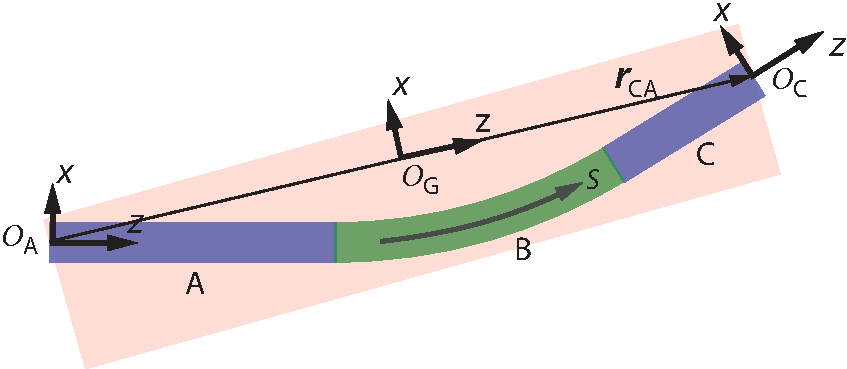
\includegraphics{girder.pdf}
  \caption[Girder example.] {
Girder supporting three elements labeled \vn{A}, \vn{B}, and \vn{C}.  $\calO_A$ is the reference
frame at the upstream end of element \vn{A} (\sref{s:ref.construct}), $\calO_C$ is the reference
frame at the downstream end of element \vn{C}, and $\calO_G$ is the default \vn{origin} reference
frame of the girder if the \vn{origin_ele} parameter is not set. $\bfr_{CA}$ is the vector from
$\calO_A$ to $\calO_C$. The length \vn{l} of the girder is set to be the difference in $s$ between
points $\calO_C$ and $\calO_A$.
  }
  \label{f:girder}
\end{figure}

A \vn{girder} is a support structure that orients the elements that are attached to it in space. A
girder can be used to simulate any rigid support structure and there are no restrictions on how the
lattice elements that are supported are oriented with respect to one another.  Thus, for example,
optical tables can be simulated.

Element parameter groups associated with this element type are:
\TOPrule
\begin{example}
  FloorParams -> Floor floor position and orientation. \sref{s:orientation.g} 
  LengthParams        -> Length and s-position parameters. \sref{s:length.g} 
  DescriptionParams   -> Element descriptive strings. \sref{s:descrip.g} 
  BodyShiftParams     -> Alignment with respect to the reference. \sref{s:alignment.g}
\end{example}
\BOTTOMrule

A simple example of a girder is shown in \fig{f:girder}. Here a girder supports three
elements labeled \vn{A}, \vn{B}, and \vn{C} where \vn{B} is a bend so the geometry is
nonlinear. Such a girder may specified in the lattice file like:
\begin{example}
  lat = Lattice(...)        # Create lattice
  create_external_ele(lat)  # Optional: Create external elements 
  @ele g1 = Girder(supported = [A, B, C], ...)
  create_girder!(g1)
\end{example}
The \vn{create_girder} command must appear after the lattice has been constructed.
The list of \vn{supported} elements must contain only elements that are in a single
lattice. Be careful here since lattice creation involves creating copies of the elments
in the \vn{BeamLines} that define the lattice. Use of the function \vn{create_external_ele}
may be useful here. The \vn{find} function may also be used to search for the appropriate
elements in the lattice. 

The list of supported elements does not have to be in any order and may contain elements from
multiple branches. A \vn{Girder} may not support slave elements.
If a super slave or multipass slave element is in the list, the slave will
be removed and the corresponding lords of the slave will be substituted into the list.

A lattice element may have at most one \vn{Girder} supporting it. However, a \vn{Girder} can be
supported by another \vn{Girder} which in turn can be supported by a third \vn{Girder}, etc. Girders
that support other Girders must be defined in the lattice file after the supported girders are
defined.

If all the supported elements of a \vn{Girder} are contained within a single lattice branch
(lord elements are considered to be in the branch(s) that their slaves are in), The length \vn{L}
of the \vn{Girder} is calculated by the difference in $s$-position from the upstream end of the
supported element with minimal $s$-position to the downstream end of the supported element with
the maximal $s$-position. If there are supported elements in multiple branches, the length is
set to \vn{NaN}. The girder length is not used in any calculations.

The reference frame from which a \vn{Girder}'s orientation is measured is set by the
\vn{origin_ele} and \vn{origin_ele_ref_point} parameters (\sref{s:origin.ele.g}).
Orientation shifts are controlled by the \vn{BodyShiftParams} (\sref{s:align.g}).

When a girder is shifted in space, the elements
it supports are also shifted.  In this case, the orientation
attributes give the orientation of
the element with respect to the \vn{girder}. The orientation with
respect to the local reference coordinates is given by
\vn{x_offset_tot}, etc, which are computed from the orientation attributes
of the element and the \vn{girder}. An example will make this clear:
\begin{example}
  q1: quad, l = 2
  q2: quad, l = 4, x_offset = 0.02, x_pitch = 0.01
  d: drift, l = 8
  g4: girder = \{q1, q2\}, x_pitch = 0.002, x_offset = 0.03
  this_line: line = (q1, d, q2)
  use, this_line
\end{example}
\index{overlay}
In this example, \vn{g4} supports quadrupoles \vn{q1} and \vn{q2}.
Since the supported elements are colinear, the computation is greatly
simplified. The reference frame of \vn{g4}, which is the default
\vn{origin} frame, is at $s = 7$~meters which is half way between the
start of \vn{q1} at at $s = 0$~meters and the end of \vn{q2}) which is
at $s = 14$. The reference frames of \vn{q1} and \vn{q2} are at their
centers so the $s$ positions of the reference frames is
\begin{example}
  Element        S_ref   dS_from_g4
  q1             1.0     -6.0
  g4             7.0      0.0
  q2            12.0      5.0
\end{example}
Using a small angle approximation to simplify the calculation, the \vn{x_pitch} of \vn{g4} produces
an offset at the center of \vn{q2} of $0.01 = 0.002 * 5$. This, added to the offsets of \vn{g4} and
\vn{q2}, give the total \vn{x_offset}, denoted \vn{x_offset_tot} of \vn{q2} is $0.06 = 0.01 + 0.03 +
0.02$. The total \vn{x_pitch}, denoted \vn{x_pitch_tot}, of \vn{q2} is $0.022 = 0.02 + 0.001$.

A \vn{Girder} that has its \vn{is_on} attribute set to False is considered to be unsifted with
respect to it's reference frame.

%---------------------------------------------------------------------------------------------------
\section{Instrument}
\label{s:instrument}

An \vn{Instrument} is like a \vn{Drift} except it represents some measurement device.

%---------------------------------------------------------------------------------------------------
\section{Kicker}
\label{s:kicker}

A \vn{Kicker} element gives particles a kick.

NOTE: This Element is in development and is incomplete.

%---------------------------------------------------------------------------------------------------
\section{LCavity}
\label{s:lcavity}

An \vn{LCavity} is a LINAC accelerating cavity.  The main difference between an \vn{RFCavity} and an
\vn{LCavity} is that, unlike an \vn{RFCavity}, the reference energy (\sref{s:ref.energy}) through
an \vn{LCavity} is not constant.

NOTE: This Element is in development and is incomplete.

%---------------------------------------------------------------------------------------------------
\section{Marker}
\label{s:marker}

A \vn{Marker} is a zero length element meant to mark a position in the machine. 

%---------------------------------------------------------------------------------------------------
\section{Mask}
\label{s:mask}

A \vn{Mask} element defines an aperture where the mask area can
essentially have an arbitrary shape. 

NOTE: This Element is in development and is incomplete.

%---------------------------------------------------------------------------------------------------
\section{Match}
\label{s:match}

A \vn{Match} element is used to adjust Twiss and orbit parameters.

NOTE: This Element is in development and is incomplete.

%---------------------------------------------------------------------------------------------------
\section{Multipole}
\label{s:mult}

A \vn{Multipole} is a thin magnetic multipole lens.

%---------------------------------------------------------------------------------------------------
\section{NullEle}
\label{s:nullele}

A \vn{NullEle} is used for bookkeeping purposes. For example, a \vn{NullEle} can be used as
the default value for a function argument or as a temporary place marker in a lattice.

%---------------------------------------------------------------------------------------------------
\section{Octupole}
\label{s:octupole}

An \vn{Octupole} is a magnetic element with a cubic field dependence
with transverse position (\sref{s:mag.field}).

%-----------------------------------------------------------------------------

\begin{figure}[bt]
  \centering
  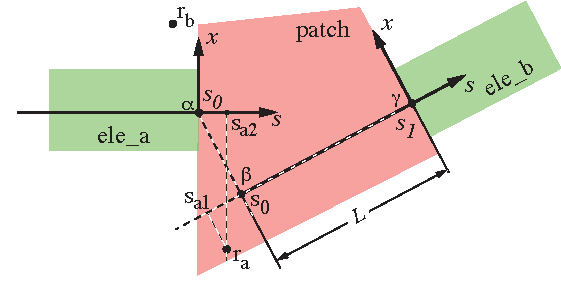
\includegraphics[width=5in]{patch-problem.pdf}
  \caption[The branch reference coordinates in a \vn{Patch} element.]
{The branch reference coordinates in a \vn{Patch} element. The \vn{Patch} element, shown
schematically as an irregular quadrilateral, is sandwiched between elements \vn{ele_a} and
\vn{ele_b}. \vn{L} is the length of the \vn{Patch}. In this example, the \vn{Patch} has a finite
\vn{y_rot}.}
  \label{f:patch.prob}
\end{figure}

%---------------------------------------------------------------------------------------------------
\section{Patch}
\label{s:patch}

A \vn{Patch} element shifts the reference orbit and time. Also see \vn{FloorShift}
(\sref{s:floorshift}) and \vn{Fiducial} (\sref{s:fiducial}) elements. A common application of a patch
is to orient two branch lines with respect to each other. 


A \vn{Patch} (\sref{s:patch}) element is different in that there is no ``natural'' coordinate 
system to use within the Patch. This is generally not an issue when the region inside the
Patch is field and aperture free since particle tracking can be done in one step from edge
to edge. However, when there are fields or apertures an internal
coordinate system is needed so that the fields or apertures can be unambiguously positioned.



%----
There 


Generally, if a particle is reasonably near the branch reference curve, there is a one-to-one mapping
between the particle's position and branch $(x, y, s)$ coordinates. 


with a non-zero \vn{x_rot} or non-zero \vn{y_rot} breaks the one-to-one mapping. This is
illustrated in \fig{f:patch.prob}.  The \vn{Patch} element, shown schematically as an, irregular
quadrilateral, is sandwiched between elements \vn{ele_a} and \vn{ele_b}. The branch coordinate system
with origin at $\alpha$ are the coordinates at the end of \vn{ele_a}. The coordinates at the end of
the \vn{Patch} has its origin labeled $\gamma$. By convention, the length of the patch \vn{L} is
taken to be the longitudinal distance from $\alpha$ to $\gamma$ with the \vn{Patch}'s exit
coordinates defining the longitudinal direction. The ``beginning'' point of the \vn{Patch} on the
reference curve a distance \vn{L} from point $\gamma$ is labeled $\beta$ in the figure.

In the branch $(x, y, s)$ coordinate system a particle at $\alpha$ will have some value $s = s_0$. A
particle at point $\beta$ will have the same value $s = s_0$ and a particle at $\gamma$ will have $s
= s_1 = s_0 + L$. A particle at point $r_a$ in \fig{f:patch.prob} illustrates the problem of
assigning $(x, y, s)$ coordinates to a given position. If the particle is considered to be within
the region of \vn{ele_a}, the particle's $s$ position will be $s_{a2}$ which is greater than the
value $s_0$ at the exit end of the element. This contradicts the expectation that particles within
\vn{ele_a} will have $s \le s_0$.  If, on the other hand, the particle is considered to be within
the \vn{Patch} region, the particle's $s$ position will be $s_{a1}$ which is less than the value
$s_0$ at the entrance to the patch. This contradicts the expectation that a particles within the
\vn{Patch} will have $s \ge s_0$.

To resolve this problem, \accellat considers a particle at position $r_a$ to be within the \vn{Patch}
region. This means that there is, in theory, no lower limit to the $s$-position that a particle in
the \vn{Patch} region can have. This also implies that there is a discontinuity in the $s$-position
of a particle crossing the exit face of \vn{ele1}. Typically, when particles are translated from the
exit face of one element to the exit face of the next, this \vn{Patch} problem does not appear. It
only appears when the track between faces is considered.

Notice that a particle at position $r_b$ in \fig{f:patch.prob} can simultaneously be considered to
be in either \vn{ele_a} or the \vn{Patch}. While this creates an ambiguity it does not complicate
tracking.

%---------------------------------------------------------------------------------------------------
\section{Quadrupole}
\label{s:quadrupole}

A \vn{Quadrupole} is a magnetic element with a linear field dependence
with transverse offset (\sref{s:mag.field}).


%---------------------------------------------------------------------------------------------------
\section{RFCavity}
\label{s:rfcavity}

An \vn{RFCavity} is an RF cavity without acceleration generally used in a storage ring. The main
difference between an \vn{RFCavity} and an \vn{LCavity} is that, unlike an \vn{Lcavity}, the
reference energy (\sref{s:phase.space}) through an \vn{RFCavity} is constant.

NOTE: This Element is in development and is incomplete.

%---------------------------------------------------------------------------------------------------
\section{Sextupole}
\label{s:sextupole}

A \vn{Sextupole} is a magnetic element with a quadratic field
dependence with transverse offset (\sref{s:mag.field}).


%---------------------------------------------------------------------------------------------------
\section{Solenoid}
\label{s:solenoid}

A \vn{solenoid} is an element with a longitudinal magnetic field.

%---------------------------------------------------------------------------------------------------
\section{Taylor}
\label{s:taylor}

A \vn{Taylor} element is a Taylor map (\sref{s:taylor.phys}) that maps the input orbital phase space and
possibly spin coordinates of a particle to the output orbital and
spin coordinates at the exit end of the element.

NOTE: This Element is in development and is incomplete.

%---------------------------------------------------------------------------------------------------
\section{ThickMultipole}
\label{s:thickmult}

A \vn{ThickMultipole} is a general non-zero length multipole element.

%---------------------------------------------------------------------------------------------------
\section{Undulator}
\label{s:undulator}

An \vn{Undulator} is and element with a periodic array of alternating bends.
Also see \vn{Wiggler} elements.

NOTE: This Element is in development and is incomplete.

%---------------------------------------------------------------------------------------------------
\section{UnionEle}
\label{s:unionele}

A \vn{UnionEle} is an element that contains a collection of other elements.
A \vn{UnionEle} is used when elements overlap spatially which happens with superposition (\sref{c:super}).

%---------------------------------------------------------------------------------------------------
\section{Wiggler}
\label{s:wiggler}

A \vn{Wiggler} is and element with a periodic array of alternating bends.
Also see \vn{Undulator} elements.

NOTE: This Element is in development and is incomplete.
